\section{tasks::test2 Class Reference}
\label{classtasks_1_1test2}\index{tasks::test2@{tasks::test2}}
Inheritance diagram for tasks::test2::\begin{figure}[H]
\begin{center}
\leavevmode
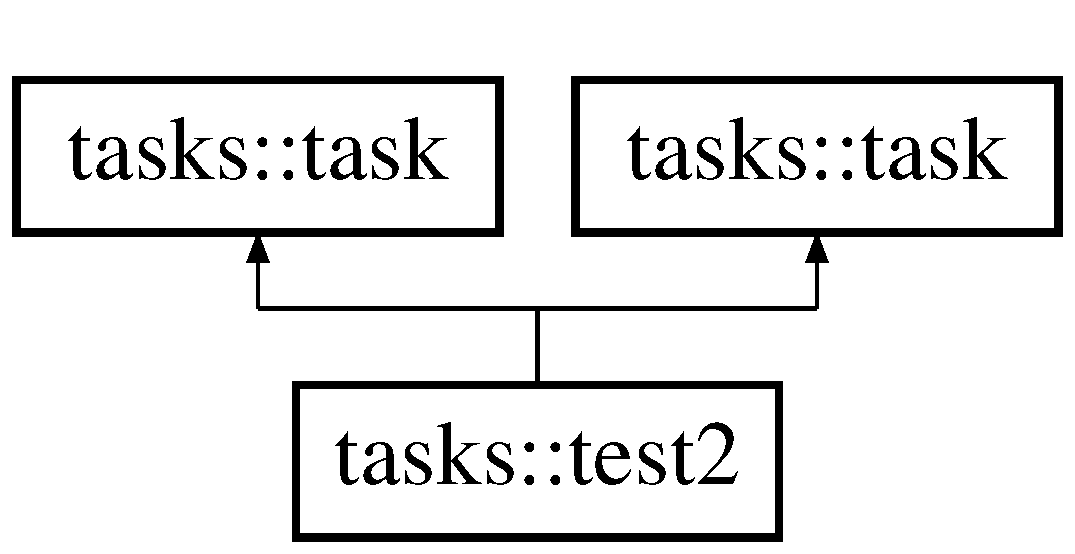
\includegraphics[height=2cm]{classtasks_1_1test2}
\end{center}
\end{figure}
\subsection*{Public Member Functions}
\begin{CompactItemize}
\item 
def \textbf{\_\-\_\-init\_\-\_\-}\label{classtasks_1_1test2_3471bd5d13ce9b406bbeaaf9ff95a276}

\item 
def \textbf{run}\label{classtasks_1_1test2_9c98ce5152399d4ff854b3da5c263354}

\item 
def \textbf{\_\-\_\-init\_\-\_\-}\label{classtasks_1_1test2_3471bd5d13ce9b406bbeaaf9ff95a276}

\item 
def \textbf{run}\label{classtasks_1_1test2_9c98ce5152399d4ff854b3da5c263354}

\end{CompactItemize}
\subsection*{Public Attributes}
\begin{CompactItemize}
\item 
\textbf{frame\_\-in}\label{classtasks_1_1test2_5f996eb068089f6bb0251020246959d8}

\item 
\textbf{frame\_\-out}\label{classtasks_1_1test2_cfdee3257fef1d67cf9c3c538abeb8ca}

\item 
\textbf{bd\-Pixel}\label{classtasks_1_1test2_16d25f922d1d5a3dc9ac52262cf2ccd1}

\end{CompactItemize}
\subsection*{Static Public Attributes}
\begin{CompactItemize}
\item 
string \textbf{name} = '{\bftest2}'\label{classtasks_1_1test2_6f30c5afb4d538f7046428a1112db228}

\item 
string \textbf{button\-Text} = '{\bftest2}'\label{classtasks_1_1test2_ff9a60ffbce17d2858d785d46fb37d64}

\end{CompactItemize}


\subsection{Detailed Description}


\footnotesize\begin{verbatim}
   A task only for tests
\end{verbatim}
\normalsize
 



The documentation for this class was generated from the following files:\begin{CompactItemize}
\item 
old/PANICtool-1.0/tasks.py\item 
old/tasks.py\end{CompactItemize}
